
\begin{abox}
	Practice set-1
\end{abox}
\begin{enumerate}
	\item A double pendulum consists of two point masses $m$ attached by strings of length $l$ as shown in the figure: The kinetic energy of the pendulum is
	{\exyear{NET/JRF(DEC-2011)}}
	\begin{figure}[H]
		\centering
		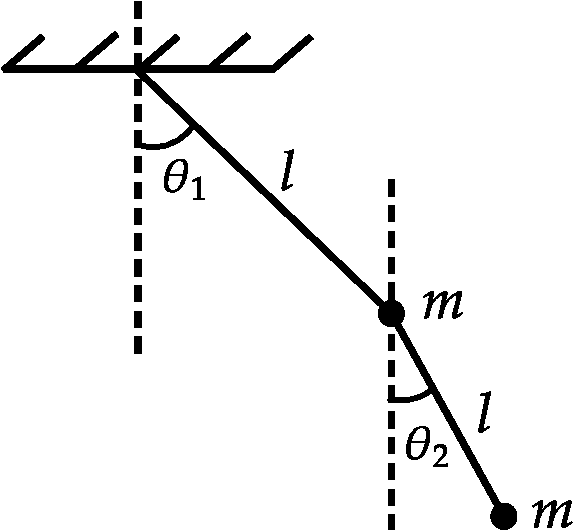
\includegraphics[height=4cm,width=4.5cm]{diagram-20210926(1)-crop}
	\end{figure}
	\begin{tasks}(1)
		\task[\textbf{A.}] $\frac{1}{2} m l^{2}\left[\dot{\theta}_{1}^{2}+\dot{\theta}_{2}^{2}\right]$
		\task[\textbf{B.}] $\frac{1}{2} m l^{2}\left[2 \dot{\theta}_{1}^{2}+\dot{\theta}_{2}^{2}+2 \dot{\theta}_{1} \dot{\theta}_{2} \cos \left(\theta_{1}-\theta_{2}\right)\right]$
		\task[\textbf{C.}] $\frac{1}{2} m l^{2}\left[\dot{\theta}_{1}^{2}+2 \dot{\theta}_{2}^{2}+2 \dot{\theta}_{1} \dot{\theta}_{2} \cos \left(\theta_{1}-\theta_{2}\right)\right]$
		\task[\textbf{D.}] $\frac{1}{2} m l^{2}\left[2 \dot{\theta}_{1}^{2}+\dot{\theta}_{2}^{2}+2 \dot{\theta}_{1} \dot{\theta}_{2} \cos \left(\theta_{1}+\theta_{2}\right)\right]$
	\end{tasks}
\begin{answer}
	\begin{align*}
	\text{	Let co-ordinate }&\left(x_{1}, y_{1}\right)\text{ and }\left(x_{2}, y_{2}\right) .\\ K . E .&=\frac{1}{2} m\left(\dot{x}_{1}^{2}+\dot{y}_{1}^{2}\right)+\frac{1}{2} m\left(\dot{x}_{2}^{2}+\dot{y}_{2}^{2}\right)\\
	x_{1}&=l \sin \theta_{1}, y_{1}=l \cos \theta_{1} \Rightarrow \dot{x}_{1}\\&=l \cos \theta_{1} \dot{\theta}_{1}, \dot{y}_{1}=-l \sin \theta_{1} \dot{\theta}_{1}\\
	x_{2}&=l \sin \theta_{1}+l \sin \theta_{2}, y_{2}=l \cos \theta_{1}+l \cos \theta_{2}\\
	\Rightarrow \dot{x}_{2}&=l \cos \theta_{1} \dot{\theta}_{1}+l \cos \theta_{2} \dot{\theta}_{2}, \dot{y}_{2}\\&=l\left(-\sin \theta_{1} \dot{\theta}_{1}\right)+l\left(-\sin \theta_{2}\right) \dot{\theta}_{2}
	\intertext{Put the value of $\dot{x}_{1}, \dot{y}_{1}, \dot{x}_{2}, \dot{y}_{2}$ in K.E equation, one will get}
	T&=\frac{1}{2} m l^{2}\left[2 \dot{\theta}_{1}^{2}+\dot{\theta}_{2}^{2}+2 \dot{\theta}_{1} \dot{\theta}_{2} \cos \left(\theta_{1}-\theta_{2}\right)\right]
	\end{align*}
	So the correct answer is \textbf{Option (B)}
\end{answer}
	\item A particle of mass $m$ moves inside a bowl. If the surface of the bowl is given by the equation $z=\frac{1}{2} a\left(x^{2}+y^{2}\right)$, where $a$ is a constant, the Lagrangian of the particle is
	{\exyear{NET/JRF(DEC-2011)}}
	\begin{tasks}(2)
		\task[\textbf{A.}] $\frac{1}{2} m\left(\dot{r}^{2}+r^{2} \dot{\phi}^{2}-g a r^{2}\right)$
		\task[\textbf{B.}] $\frac{1}{2} m\left[\left(1+a^{2} r^{2}\right) \dot{r}^{2}+r^{2} \dot{\phi}^{2}\right]$
		\task[\textbf{C.}]  $\frac{1}{2} m\left(\dot{r}^{2}+r^{2} \dot{\theta}^{2}+r^{2} \sin ^{2} \theta \dot{\phi}^{2}-g a r^{2}\right)$
		\task[\textbf{D.}]  $\frac{1}{2} m\left[\left(1+a^{2} r^{2}\right) \dot{r}^{2}+r^{2} \dot{\phi}^{2}-g a r^{2}\right]$
	\end{tasks}
\begin{answer}
	\begin{align*}
	L&=\frac{1}{2} m\left(\dot{x}^{2}+\dot{y}^{2}+\dot{z}^{2}\right)-m g z,\\\text{ where } z&=\frac{1}{2} a\left(x^{2}+y^{2}\right)\\
	\text{It has cylindrical symmetry. Thus }x&=r \cos \phi, y=r \sin \phi, z=\frac{1}{2} a\left(r^{2}\right)\\
	\dot{x}&=\dot{r} \cos \phi-r \sin \phi \dot{\phi}, \dot{y}\\&=\dot{r} \sin \phi+r \cos \phi \dot{\phi}\text{ and }\dot{z}=a(r \dot{r})\\
	\text{	So, }L&=\frac{1}{2} m\left[\left(1+a^{2} r^{2}\right) \dot{r}^{2}+r^{2} \dot{\phi}^{2}-g a r^{2}\right]
	\end{align*}
	So the correct answer is \textbf{Option (D)}
\end{answer}
	\item The Lagrangian of a particle of mass $m$ moving in one dimension is given by
	$$
	L=\frac{1}{2} m \dot{x}^{2}-b x
	$$
	where $b$ is a positive constant. The coordinate of the particle $x(t)$ at time $t$ is given by: (in following $c_{1}$ and $c_{2}$ are constants)
	{\exyear{NET/JRF(JUNE-2013)}}
	\begin{tasks}(2)
		\task[\textbf{A.}] $-\frac{b}{2 m} t^{2}+c_{1} t+c_{2}$
		\task[\textbf{B.}] $c_{1} t+c_{2}$
		\task[\textbf{C.}] $c_{1} \cos \left(\frac{b t}{m}\right)+c_{2} \sin \left(\frac{b t}{m}\right)$
		\task[\textbf{D.}] $c_{1} \cosh \left(\frac{b t}{m}\right)+c_{2} \sinh \left(\frac{b t}{m}\right)$
	\end{tasks}	
\begin{answer}
	\begin{align*}
	\text{Equation of motion }\frac{d}{d t}\left(\frac{\partial L}{\partial \dot{x}}\right)-\frac{\partial L}{\partial x}&=0 \Rightarrow \frac{d}{d t}(m \dot{x})+b\\&=0 \Rightarrow m \ddot{x}+b=0 \Rightarrow m \ddot{x}=-b\\
	\frac{d^{2} x}{d t^{2}}&=-\frac{b}{m} \Rightarrow \frac{d x}{d t}=-\frac{b}{m} t+c_{1} \Rightarrow x\\&=-\frac{b}{m} \frac{t^{2}}{2}+c_{1} t+c_{2}
	\end{align*}
	So the correct answer is \textbf{Option (A)}
\end{answer}
	\item A particle moves in a potential $V=x^{2}+y^{2}+\frac{z^{2}}{2} .$ Which component(s) of the angular momentum is/are constant(s) of motion?
	{\exyear{NET/JRF(DEC-2013)}}
	\begin{tasks}(4)
		\task[\textbf{A.}] None
		\task[\textbf{B.}] $L_{x}, L_{y}$ and $L_{z}$
		\task[\textbf{C.}]  only $L_{x}$ and $L_{y}$
		\task[\textbf{D.}] only $L_{z}$
	\end{tasks}
\begin{answer}
	\begin{align*}
	\text{A particle moves in a potential }V&=x^{2}+y^{2}+\frac{z^{2}}{2}\\
	V(r, \theta, \phi)&=r^{2} \sin ^{2} \theta \cos ^{2} \phi+r^{2} \sin ^{2} \theta \sin ^{2} \phi+\frac{r^{2}}{2} \cos ^{2} \theta\\
	V(r, \theta, \phi)&=r^{2} \sin ^{2} \theta+\frac{r^{2}}{2} \cos ^{2} \theta\\
	\text{	Now $\phi$ is cyclic-co-ordinate }&\left(p_{\phi}\right)\text{ i.e $L_{z}$ is constant of motion.}
	\end{align*}
	So the correct answer is \textbf{Option (D)}
\end{answer}
	\item A pendulum consists of a ring of mass $M$ and radius $R$ suspended by a massless rigid rod of length $l$ attached to its rim. When the pendulum oscillates in the plane of the ring, the time period of oscillation is
	{\exyear{NET/JRF(DEC-2013)}}
	\begin{tasks}(2)
		\task[\textbf{A.}] $2 \pi \sqrt{\frac{l+R}{g}}$
		\task[\textbf{B.}] $\frac{2 \pi}{\sqrt{g}}\left(l^{2}+R^{2}\right)^{1 / 4}$
		\task[\textbf{C.}] $2 \pi \sqrt{\frac{2 R^{2}+2 R l+l^{2}}{g(R+l)}}$
		\task[\textbf{D.}] $\frac{2 \pi}{\sqrt{g}}\left(2 R^{2}+2 R l+l^{2}\right)^{1 / 4}$
	\end{tasks}	
\begin{answer}
	\begin{align*}
	\intertext{The moment of inertia about pivotal point is given by}
	I&=I_{c, m}+M d^{2}=M R^{2}+M(l+R)^{2}\\
	\intertext{If ring is displaced by angle $\theta$ then potential energy is $-M g(l+R) \cos \theta$.}
	\intertext{ The Lagrangian is given by}
	L&=\frac{1}{2} I \dot{\theta}^{2}-V(\theta)\\&=\frac{1}{2}\left(M R^{2}+M(l+R)^{2}\right) \dot{\theta}^{2}+M g(l+R) \cos \theta\\
	\frac{d}{d t}\left(\frac{\partial L}{\partial \dot{\theta}}\right)-\left(\frac{\partial L}{\partial \theta}\right)&=0 \Rightarrow\left(M R^{2}+M(l+R)^{2}\right) \ddot{\theta}+M g(l+R) \sin \theta=0\\
	\text{For small oscillation }\sin \theta&=\theta \Rightarrow\left(M R^{2}+M(l+R)^{2}\right) \ddot{\theta}+M g(l+R) \theta=0\\
	\text{Time period is given by }&2 \pi \sqrt{\frac{2 R^{2}+2 R l+l^{2}}{g(R+l)}}.
	\end{align*}
	So the correct answer is \textbf{Option (C)}
\end{answer}
	\item Consider a particle of mass $m$ attached to two identical springs each of length $l$ and spring constant $k$ (see the figure). The equilibrium configuration is the one where the springs are unstretched. There are no other external forces on the system. If the particle is given a small displacement along the $x$-axis, which of the following describes the equation of motion for small oscillations?
	{\exyear{NET/JRF(DEC-2013)}}
	\begin{figure}[H]
		\centering
		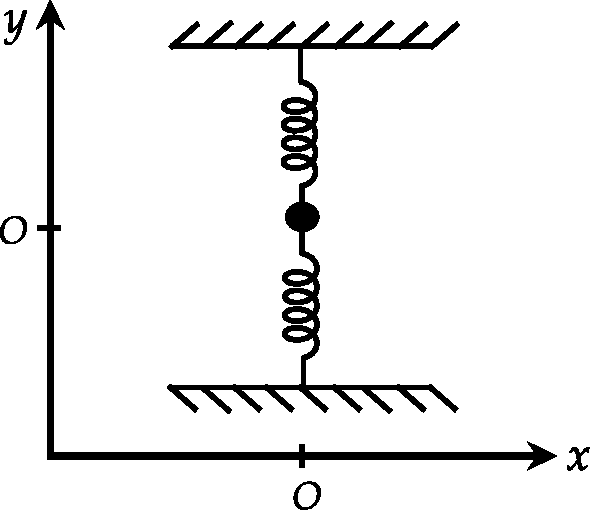
\includegraphics[height=4.5cm,width=5cm]{diagram-20210926(18)-crop}
	\end{figure}
	\begin{tasks}(4)
		\task[\textbf{A.}] $m \ddot{x}+\frac{k x^{3}}{l^{2}}=0$
		\task[\textbf{B.}]  $m \ddot{x}+k x=0$
		\task[\textbf{C.}] $m \ddot{x}+2 k x=0$
		\task[\textbf{D.}] $m \ddot{x}+\frac{k x^{2}}{l}=0$
	\end{tasks}	
\begin{answer}$\left. \right. $
	\begin{figure}[H]
		\centering
		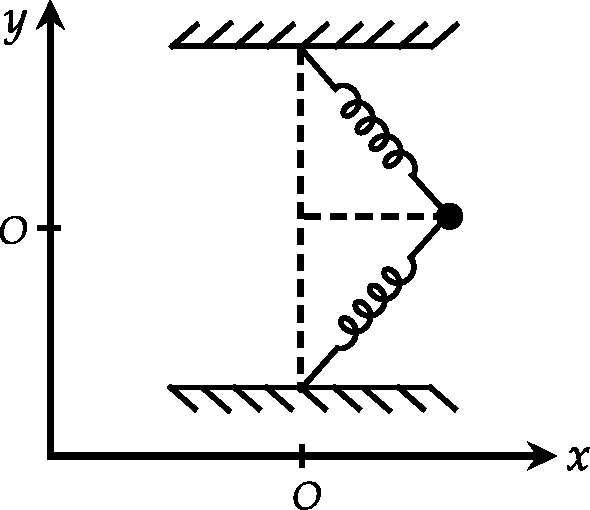
\includegraphics[height=4.5cm,width=5cm]{diagram-20210926(19)-crop}
	\end{figure}
	\begin{align*}
	\intertext{The lagrangian of system is given by}
	L&=\frac{1}{2} m \dot{x}^{2}-V(x)
	\intertext{The potential energy is given by}
	V(x)&=\frac{k}{2}\left[\left(x^{2}+l^{2}\right)^{\frac{1}{2}}-l\right]^{2}+\frac{k}{2}\left[\left(x^{2}+l^{2}\right)^{\frac{1}{2}}-l\right]^{2}\\
	V(x)&=k\left[\left(x^{2}+l^{2}\right)^{\frac{1}{2}}-l\right]^{2}
	\intertext{For small oscillation one can approximate potential by Taylor expansion}
	V(x)&=k l^{2}\left[\left(1+\frac{x^{2}}{l^{2}}\right)^{\frac{1}{2}}-1\right]^{2} \Rightarrow V(x)\\&=k l^{2}\left[\left(1+\frac{1}{2} \frac{x^{2}}{l^{2}}-\frac{1}{8} \frac{x^{4}}{l^{4}}\right)-1\right]^{2}\\
	V(x)&=\frac{k l^{2}}{4}\left(\frac{x^{2}}{l^{2}}\right)^{2} \Rightarrow V(x)=k\left(\frac{x^{4}}{4 l^{2}}\right)\\
	\text{So Lagrangian of system is given by }L&=\frac{1}{2} m \dot{x}^{2}-k\left(\frac{x^{4}}{4 l^{2}}\right)\\
	\text{The Lagranges equation of motion }&\frac{d}{d t}\left(\frac{\partial L}{\partial \dot{x}}\right)-\left(\frac{\partial L}{\partial x}\right)=0 \Rightarrow m \ddot{x}+\frac{k x^{3}}{l^{2}}=0
	\end{align*}
	So the correct answer is \textbf{Option (A)}
\end{answer}
	\item The equation of motion of a system described by the time-dependent Lagrangian
	$$
	L=e^{\gamma t}\left[\frac{1}{2} m \dot{x}^{2}-V(x)\right] \text { is }
	$$
	{\exyear{NET/JRF(DEC-2014)}}
	\begin{tasks}(2)
		\task[\textbf{A.}] $m \ddot{x}+\gamma m \dot{x}+\frac{d V}{d x}=0$
		\task[\textbf{B.}] $m \ddot{x}+\gamma m \dot{x}-\frac{d V}{d x}=0$
		\task[\textbf{C.}]  $m \ddot{x}-\gamma m \dot{x}+\frac{d V}{d x}=0$
		\task[\textbf{D.}] $m \ddot{x}+\frac{d V}{d x}=0$
	\end{tasks}
\begin{answer}
	\begin{align*}
	\because L&=e^{\gamma t}\left[\frac{1}{2} m \dot{x}^{2}-V(x)\right] \Rightarrow \frac{\partial L}{\partial \dot{x}}\\&=e^{\gamma t} m \dot{x}\text{ and }\frac{\partial L}{\partial x}=-\frac{\partial V}{\partial x} e^{\gamma t}\\
	\because \frac{d}{d t}\left(\frac{\partial L}{\partial \dot{x}}\right)-\frac{\partial L}{\partial x}&=0 \Rightarrow \frac{d}{d t}\left(e^{\gamma t} m \dot{x}\right)+\frac{\partial V}{\partial x} e^{\gamma t}\\&=m \ddot{x} e^{r t}+m \dot{x} \gamma e^{\gamma t}+\frac{\partial V}{\partial x} e^{r t}=0\\
	\left(m \ddot{x}+m \gamma \dot{x}+\frac{\partial V}{\partial x}\right) e^{\gamma t}&=0 \Rightarrow m \ddot{x}+\gamma m \dot{x}+\frac{\partial V}{\partial x}=0
	\end{align*}
	So the correct answer is \textbf{Option (A)}
\end{answer}
	\item A particle of unit mass moves in the $x y$-plane in such a way that $\dot{x}(t)=y(t)$ and $\dot{y}(t)=-x(t) .$ We can conclude that it is in a conservative force-field which can be derived from the potential
	{\exyear{NET/JRF(JUNE-2015)}}
	\begin{tasks}(4)
		\task[\textbf{A.}] $\frac{1}{2}\left(x^{2}+y^{2}\right)$
		\task[\textbf{B.}] $\frac{1}{2}\left(x^{2}-y^{2}\right)$
		\task[\textbf{C.}] $x+y$
		\task[\textbf{D.}] $x-y$
	\end{tasks}	
\begin{answer}
	\begin{align*}
	\because \dot{x}&=y\text{ and }\dot{y}=-x\\
	\Rightarrow \quad \ddot{x}&=\dot{y}=-x \quad\text{ and }\ddot{y}=-\dot{x}=-y\\
	\Rightarrow \quad \ddot{x}+x&=0 \quad\text{ and }\ddot{y}+y=0\\
	\text{that is possible for }L&=\frac{1}{2} m \dot{x}^{2}+\frac{1}{2} m \dot{y}^{2}-\frac{1}{2}\left(x^{2}+y^{2}\right) \\\Rightarrow V&=\frac{1}{2}\left(x^{2}+y^{2}\right)
	\end{align*}
	So the correct answer is \textbf{Option (A)}
\end{answer}
	\item The Lagrangian of a particle moving in a plane s given in Cartesian coordinates as
	$$
	L=\dot{x} \dot{y}-x^{2}-y^{2}
	$$
	In polar coordinates the expression for the canonical momentum $p_{r}$ (conjugate to the radial coordinate $r$ ) is
	{\exyear{NET/JRF(DEC-2015)}}
	\begin{tasks}(2)
		\task[\textbf{A.}] $\dot{r} \sin \theta+r \dot{\theta} \cos \theta$
		\task[\textbf{B.}]  $\dot{r} \cos \theta+r \dot{\theta} \sin \theta$
		\task[\textbf{C.}] $2 \dot{r} \cos \theta-r \dot{\theta} \sin 2 \theta$
		\task[\textbf{D.}] $\dot{r} \sin 2 \theta+r \dot{\theta} \cos 2 \theta$
	\end{tasks}
\begin{answer}
	\begin{align*}
	L&=\dot{x} \dot{y}-x^{2}-y^{2}=\dot{x} \dot{y}-\left(x^{2}+y^{2}\right)\\
	x&=r \cos \theta, y=r \sin \theta \Rightarrow \dot{x}=\dot{r} \cos \theta-r \sin \theta \dot{\theta}, \\ \dot{y}&=\dot{r} \sin \theta+r \cos \theta \dot{\theta}\\
	L&=\dot{r}^{2} \sin \theta \cos \theta-r^{2} \sin \theta \cos \theta \dot{\theta}^{2}+\dot{r} r \cos ^{2} \theta \dot{\theta}-\dot{r} r \sin ^{2} \theta \dot{\theta}\\
	P_{r}&=\frac{\partial L}{\partial \dot{r}} \Rightarrow 2 \dot{r} \sin \theta \cos \theta+r \dot{\theta}\left(\cos ^{2} \theta-\sin ^{2} \theta\right)\\
	\Rightarrow P_{r}&=\dot{r} \sin 2 \theta+r \dot{\theta} \cos 2 \theta
	\end{align*}
	So the correct answer is \textbf{Option (D)}
\end{answer}
	\item The dynamics of a particle governed by the Lagrangian
	$$
	L=\frac{1}{2} m \dot{x}^{2}-\frac{1}{2} k x^{2}-k x \dot{x} t \text { describes }
	$$
	{\exyear{NET/JRF(DEC-2016)}}
	\begin{tasks}(1)
		\task[\textbf{A.}] An undamped simple harmonic oscillator
		\task[\textbf{B.}] A damped harmonic oscillator with a time varying damping factor
		\task[\textbf{C.}]  An undamped harmonic oscillator with a time dependent frequency
		\task[\textbf{D.}] A free particle
	\end{tasks}	
\begin{answer}
	\begin{align*}
	L&=\frac{1}{2} m \dot{x}^{2}-\frac{1}{2} k x^{2}-k x \dot{x} t\\
	\frac{\partial L}{\partial \dot{x}}&=m \dot{x}-k x t, \frac{\partial L}{\partial x}=-k x-k \dot{x} t\\
	\frac{d}{d t}\left(\frac{\partial L}{\partial \dot{x}}\right)-\frac{\partial L}{\partial x}&=0 \Rightarrow m \ddot{x}-k \dot{x} t-k x+k x+k \dot{x} t\\&=0 \Rightarrow m \ddot{x}=0
	\intertext{So motion is equivalent to free particle}
	\end{align*}
	So the correct answer is \textbf{Option (D)}
\end{answer}
	\item The parabolic coordinates $(\xi, \eta)$ are related to the Cartesian coordinates $(x, y)$ by $x=\xi \eta$ and $y=\frac{1}{2}\left(\xi^{2}-\eta^{2}\right)$. The Lagrangian of a two-dimensional simple harmonic oscillator of mass $m$ and angular frequency $\omega$ is
	{\exyear{NET/JRF(DEC-2016)}}
	\begin{tasks}(1)
		\task[\textbf{A.}] $\frac{1}{2} m\left[\dot{\xi}^{2}+\dot{\eta}^{2}-\omega^{2}\left(\xi^{2}+\eta^{2}\right)\right]$
		\task[\textbf{B.}] $\frac{1}{2} m\left(\xi^{2}+\eta^{2}\right)\left[\left(\dot{\xi}^{2}+\dot{\eta}^{2}\right)-\frac{1}{4} \omega^{2}\left(\xi^{2}+\eta^{2}\right)\right]$
		\task[\textbf{C.}] $\frac{1}{2} m\left(\xi^{2}+\eta^{2}\right)\left[\dot{\xi}^{2}+\dot{\eta}^{2}-\frac{1}{2} \omega^{2} \xi \eta\right]$
		\task[\textbf{D.}] $\frac{1}{2} m\left(\xi^{2}+\eta^{2}\right)\left[\dot{\xi}^{2}+\dot{\eta}^{2}-\frac{1}{4} \omega^{2}\right]$
	\end{tasks}	
\begin{answer}
	\begin{align*}
	\intertext{For two dimensional Harmonic oscillation}
	L&=\frac{1}{2} m\left(\dot{x}^{2}+\dot{y}^{2}\right)-\frac{1}{2} m \omega^{2}\left(x^{2}+y^{2}\right)\\
	x&=\xi \eta, \quad y=\frac{1}{2}\left(\xi^{2}-\eta^{2}\right)\\
	\dot{x}&=\dot{\xi} \eta+\xi \dot{\eta}, \quad \dot{y}=\xi \dot{\xi}-\eta \dot{\eta}\\
	L&=\frac{1}{2} m\left[(\dot{\xi} \eta+\xi \dot{\eta})^{2}+(\xi \dot{\xi}-\eta \dot{\eta})^{2}\right]-\frac{1}{2} m \omega^{2}\left[\xi^{2} \eta^{2}+\frac{1}{4}\left(\xi^{2}-\eta^{2}\right)^{2}\right]\\
	L&=\frac{1}{2} m\left(\dot{\xi}^{2} \eta^{2}+\xi^{2} \dot{\eta}^{2}+\xi^{2} \dot{\xi}^{2}+\eta^{2} \dot{\eta}^{2}\right)-\frac{1}{8} m \omega^{2}\left(\xi^{4}+\eta^{4}+2 \xi^{2} \eta^{2}\right)\\
	&=\frac{1}{2} m\left(\xi^{2}+\eta^{2}\right)\left(\dot{\eta}^{2}+\dot{\xi}^{2}\right)-\frac{1}{8} m \omega^{2}\left(\xi^{2}+\eta^{2}\right)^{2}\\
	&=\frac{1}{2} m\left(\xi^{2}+\eta^{2}\right)\left[\dot{\eta}^{2}+\dot{\xi}^{2}-\frac{1}{4} \omega^{2}\left(\xi^{2}+\eta^{2}\right)\right]
	\end{align*}
	So the correct answer is \textbf{Option (B)}
\end{answer}
	\item The spring constant $k$ of a spring of mass $m_{s}$ is determined experimentally by loading the spring with mass $M$ and recording the time period $T$, for a single oscillation. If the experiment is carried out for different masses, then the graph that correctly represents the result is
	{\exyear{NET/JRF(DEC-2017)}}
	\begin{tasks}(2)
		\task[\textbf{A.}] \begin{figure}[H]
			\centering
			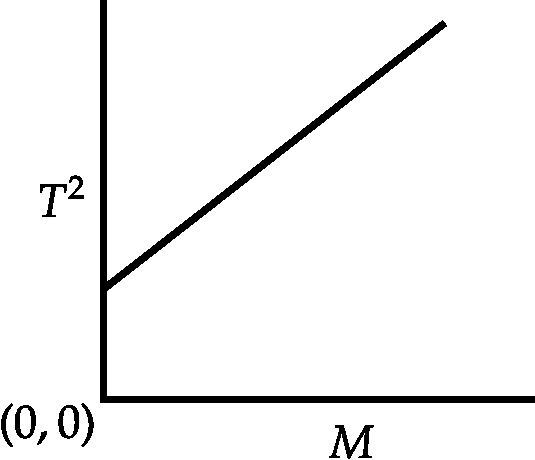
\includegraphics[height=3cm,width=3.5cm]{diagram-20210926(38)-crop}
		\end{figure}
		\task[\textbf{B.}] \begin{figure}[H]
			\centering
			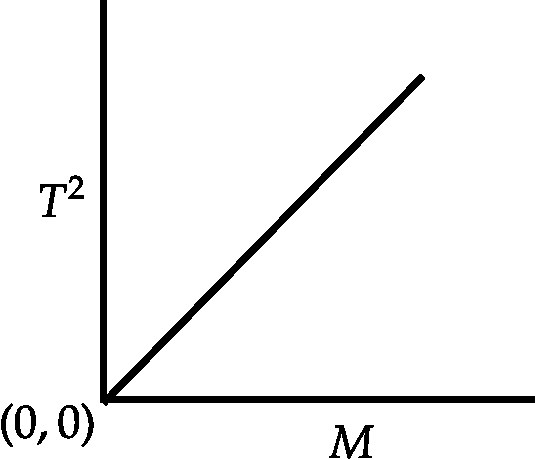
\includegraphics[height=3cm,width=3.5cm]{diagram-20210926(39)-crop}
		\end{figure}
		\task[\textbf{C.}] \begin{figure}[H]
			\centering
			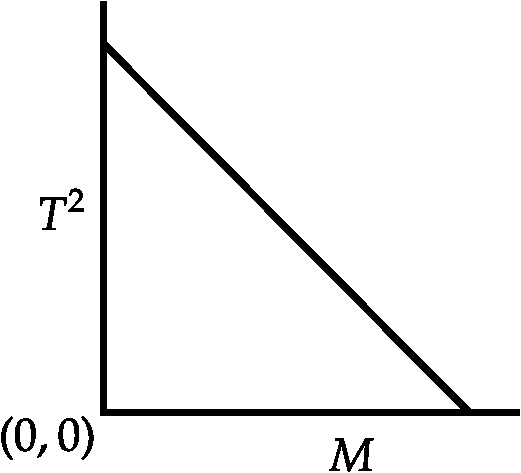
\includegraphics[height=3cm,width=3.5cm]{diagram-20210926(40)-crop}
		\end{figure}
		\task[\textbf{D.}] \begin{figure}[H]
			\centering
			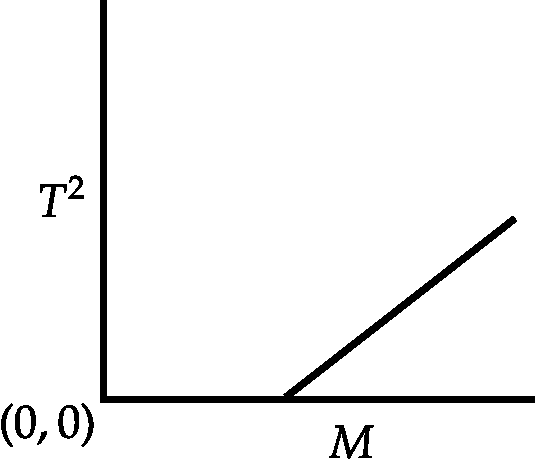
\includegraphics[height=3cm,width=3.5cm]{diagram-20210926(41)-crop}
		\end{figure}
	\end{tasks}	
\begin{answer}
	\begin{align*}
	\intertext{The Langrangian of system.}
	L&=\frac{1}{2} \cdot \frac{m_{s}}{3} \dot{x}^{2}+\frac{1}{2} M \dot{x}^{2}-\frac{1}{2} k x^{2}, \frac{d}{d t}\left(\frac{\partial L}{\partial \dot{x}}\right)-\frac{\partial L}{\partial x}=0\\
	\frac{d}{d t} \frac{\partial L}{\partial x}&=0 \Rightarrow\left(\frac{m_{s}}{3}+M\right) \ddot{x}=-k x\\
	T&=2 \pi \sqrt{\frac{M+\frac{m_{s}}{3}}{k}} \Rightarrow T^{2}=4 \pi \frac{\left(M+\frac{m_{s}}{3}\right)}{k}
	\end{align*}
	So the correct answer is \textbf{Option (A)}
\end{answer}
	\item The motion of a particle in one dimension is described by the Langrangian $L=\frac{1}{2}\left(\left(\frac{d x}{d t}\right)^{2}-x^{2}\right)$ in suitable units. The value of the action along the classical path from $x=0$ at $t=0$ to $x=x_{0}$ at $t=t_{0}$, is
	{\exyear{NET/JRF(DEC-2018)}}
	\begin{tasks}(4)
		\task[\textbf{A.}] $\frac{x_{0}^{2}}{2 \sin ^{2} t_{0}}$
		\task[\textbf{B.}] $\frac{1}{2} x_{0}^{2} \tan t_{0}$
		\task[\textbf{C.}] $\frac{1}{2} x_{0}^{2} \cot t_{0}$
		\task[\textbf{D.}] $\frac{x_{0}^{2}}{2 \cos ^{2} t_{0}}$
	\end{tasks}	
\begin{answer}
	\begin{align*}
	L&=\frac{1}{2} \dot{x}^{2}-\frac{1}{2} x^{2}\\
	\intertext{From Lagrangian equation of motion, $\frac{d}{d t}\left(\frac{\partial L}{\partial \dot{x}}\right)-\frac{\partial L}{\partial x}=0$}
	\ddot{x}+x&=0\\
	\text{The solution is}&=A \sin t+B \cos t\\
	t&=0, \quad x=0, \quad B=0\\
	x&=A \sin t\\
	t&=t_{0}, \quad x=x_{0}, A=\frac{x_{0}}{\sin t_{0}}\\
	x&=\frac{x_{0}}{\sin t_{0}} \sin t, \quad \dot{x}=\frac{x_{0}}{\sin t_{0}} \cos t\\
	A&=\int_{0}^{t_{0}} L d t=\int_{0}^{t_{0}} \frac{1}{2} \dot{x}^{2} d t-\int_{0}^{t_{0}} \frac{1}{2} x^{2} d t\\&=\frac{1}{2} \frac{x_{0}^{2}}{\sin ^{2} t_{0}} \int_{0}^{t_{0}} \cos ^{2} t d t-\frac{1}{2} \frac{x_{0}^{2}}{\sin ^{2} t_{0}} \int_{0}^{t_{0}} \sin ^{2} t d t\\
	&=\frac{1}{2} \frac{x_{0}^{2}}{\sin ^{2} t_{0}}\left[\int_{0}^{t_{0}} \cos ^{2} t d t-\int_{0}^{t} \sin ^{2} t d t\right]\\&=\frac{1}{2} \frac{x_{0}^{2}}{\sin ^{2} t_{0}} \int_{t}^{t_{0}} \cos 2 t d t=\left.\frac{1}{2} \frac{x_{0}^{2}}{\sin ^{2} t_{0}} \frac{\sin 2 t_{0}}{2}\right|_{0} ^{t_{0}}=\frac{x_{0}^{2}}{2} \cot t_{0}
	\end{align*}
	So the correct answer is \textbf{Option (C)}
\end{answer}
	\item Two particles of masses $m_{1}$ and $m_{2}$ are connected by a massless thread of length $l$ as shown in figure below.\\
	The particle of mass in on the plane undergoes a circular motion with radius $r_{0}$ and angular momentum $L$. When a small radial displacement $\in$ (whew $\in \ll<r_{0}$ ) is applied, its radial coordinate is found to oscillate about $r_{0}$. The frequency of the oscillations is
	{\exyear{NET/JRF(JUNE-2019)}}
	\begin{tasks}(4)
		\task[\textbf{A.}] $\sqrt{\frac{7 m_{2} g}{\left(m_{1}+\frac{m_{2}}{2}\right) r_{0}}}$
		\task[\textbf{B.}] $\sqrt{\frac{7 m_{2} g}{\left(m_{1}+m_{2}\right) r_{0}}}$
		\task[\textbf{C.}] $\sqrt{\frac{3 m_{2} g}{\left(m_{1}+\frac{m_{2}}{2}\right) r_{0}}}$
		\task[\textbf{D.}] $\sqrt{\frac{3 m_{2} g}{\left(m_{1}+m_{2}\right) r_{0}}}$
	\end{tasks}
\begin{answer}
	\begin{align*}
	L&=\frac{1}{2}\left(m_{1}+m_{2}\right) \ddot{r}+\frac{1}{2} m_{1} r^{2} \dot{\theta}^{2}-m_{2} g(l-r)\\
	\text{Lagrangian equation of motion; }&\frac{d}{d t}\left(\frac{\partial L}{\partial \dot{r}}\right)-\frac{\partial L}{\partial r}=0\\
	\left(m_{1}+m_{2}\right) \ddot{r}-m_{1} r \dot{\theta}^{2}+m_{2} g&=0
	\intertext{Hence angular momentum is conserved}
	m_{1} r^{2} \dot{\theta}&=m_{1} r_{0}^{2} \dot{\theta}_{0} \Rightarrow \dot{\theta}=\frac{r_{0}^{2} \dot{\theta}_{0}}{r^{2}}\\
	\text{For circular motion }&m r_{0} \dot{\theta}_{0}^{2}=m_{2} g\\
	\text{	so }r \dot{\theta}^{2}&=\frac{m_{2}}{m_{1}}\left(\frac{r_{0}}{r}\right)^{3} g\\
	\left(m_{1}+m_{2}\right) \ddot{r}-m_{2}\left(\frac{r_{0}}{r}\right)^{3} g+m_{2} g&=0\\
	\text{Put }r&=r_{0}+\in \ddot{r}=\ddot{\epsilon}\\
	\intertext{$\left(m_{1}+m_{2}\right) \ddot{\in}-m_{2}\left(\frac{r_{0}}{r_{0}+\epsilon}\right)^{3} g+m_{2} g\Rightarrow\left(m_{1}+m_{2}\right) \ddot{\in}-m_{2} r_{0}^{3}\left(r_{0}+\epsilon\right)^{-3} g+m_{2} g$}\\
	\left(m_{1}+m_{2}\right) \ddot{\star}-m_{2} r_{0}^{3} g r_{0}^{-3}\left(1+\frac{\epsilon}{r_{0}}\right)^{-3}+m_{2} g&=0\\
	\left(m_{1}+m_{2}\right) \ddot+\frac{m_{2} 3 \epsilon}{r_{0}}&=0 \Rightarrow \omega=\sqrt{\frac{3 m_{2} g}{\left(m_{1}+m_{2}\right) r_{0}}}
	\end{align*}
	So the correct answer is \textbf{Option (D)}
\end{answer}	
	\item Which of the following terms, when added to the Lagrangian $L(x, y, \dot{x}, \dot{y})$ of a system with two degrees of freedom will not change the equations of motion?\\
	(check question )
	{\exyear{NET/JRF(DEC-2019)}}
	\begin{tasks}(4)
		\task[\textbf{A.}] $x \ddot{x}-y \ddot{y}$
		\task[\textbf{B.}] $x \ddot{y}-y \ddot{x}$
		\task[\textbf{C.}] $x \dot{y}-y \dot{x}$
		\task[\textbf{D.}] $y \dot{x}^{2}+x \dot{y}^{2}$ 
	\end{tasks}
\begin{answer}
	\begin{align*}
	L(x, y, \dot{x}, \dot{y})\\
	\frac{d}{d t}\left(\frac{\partial L}{\partial \dot{x}}\right)-\frac{\partial L}{\partial x}&=0, \frac{d}{d t}\left(\frac{\partial L}{\partial \dot{y}}\right)-\frac{\partial L}{\partial y}=0\\
	L^{\prime}&=L(x, y, \dot{x}, \dot{y})+x \ddot{y}-y \ddot{x}\\
	\frac{d^{\prime}}{d t^{\prime}}\left(\frac{\partial L^{\prime}}{\partial \dot{x}}\right)-\frac{\partial L^{\prime}}{\partial x}&=\frac{d}{d t}\left(\frac{\partial L}{\partial \dot{x}}\right)-\frac{\partial L}{\partial x}+\ddot{y}\\&=0=0+\ddot{y}=0 \Rightarrow \dot{y}=c_{1}\\
	\frac{d}{d t}\left(\frac{\partial L}{\partial y}\right)-\frac{\partial L^{\prime}}{\partial y}&=\frac{d}{d t}\left(\frac{\partial L}{\partial \dot{y}}\right)-\frac{\partial L}{\partial y}+\ddot{x}\\&=0=0-\ddot{x}=0 \Rightarrow \dot{x}=c_{2}
	\end{align*}
	So the correct answer is \textbf{Option (B)}
\end{answer}
	\item A point mass $m$, is constrained to move on the inner surface of a paraboloid of revolution $x^{2}+y^{2}=a z$ (where $a>0$ is a constant). When it spirals down the surface, under the influence of gravity (along $-z$ direction), the angular speed about the $z$-axis is proportional to
	{\exyear{NET/JRF(JUNE-2020)}}
	\begin{tasks}(2)
		\task[\textbf{A.}] 1 (independent of $z$ )
		\task[\textbf{B.}] $z$
		\task[\textbf{C.}]  $z^{-1}$
		\task[\textbf{D.}] $z^{-2}$
	\end{tasks}	
\begin{answer}
	\begin{align*}
	\intertext{Using Lagrangian in cylindrical coordinate}
	L&=\frac{1}{2} m\left(\dot{r}^{2}+r^{2} \dot{\theta}^{2}+\dot{z}^{2}\right)-m g z \\\text{ with constraint }x^{2}+y^{2}&=a z \Rightarrow r^{2}=a z \Rightarrow \dot{z}=\frac{2 r \dot{r}}{a}\\
	L&=\frac{1}{2} m\left(\dot{r}^{2}+r^{2} \dot{\theta}^{2}+\left(\frac{2 r \dot{r}}{a}\right)^{2}\right)-\frac{m g r^{2}}{a}\\
	\theta \text{is cyclic coordinate so }\frac{\partial L}{\partial \theta}&=0 \Rightarrow \frac{\partial L}{\partial \dot{\theta}}=J \Rightarrow m r^{2} \dot{\theta}=J \Rightarrow \dot{\theta} \propto \frac{1}{r^{2}} \propto \frac{1}{z}
	\end{align*}
	So the correct answer is \textbf{Option (C)}
\end{answer}
\end{enumerate}
\colorlet{ocre1}{ocre!70!}
\colorlet{ocrel}{ocre!30!}
\setlength\arrayrulewidth{1pt}
\begin{table}[H]
	\centering
	\arrayrulecolor{ocre}
	\begin{tabular}{|p{1.5cm}|p{1.5cm}||p{1.5cm}|p{1.5cm}|}
		\hline
		\multicolumn{4}{|c|}{\textbf{Answer key}}\\\hline\hline
		\rowcolor{ocrel}Q.No.&Answer&Q.No.&Answer\\\hline
		1&\textbf{B} &2&\textbf{D}\\\hline 
		3&\textbf{A} &4&\textbf{D} \\\hline
		5&\textbf{C} &6&\textbf{A} \\\hline
		7&\textbf{A}&8&\textbf{A}\\\hline
		9&\textbf{D}&10&\textbf{D}\\\hline
		11&\textbf{B} &12&\textbf{A}\\\hline
		13&\textbf{C}&14&\textbf{D}\\\hline
		15&\textbf{B}&16&\textbf{C}\\\hline
		
	\end{tabular}
\end{table}
\newpage
\begin{abox}
	Practice set-2
\end{abox}
\begin{enumerate}
	\item A particle of mass $m$ slides under the gravity without friction along the parabolic path $y=a x^{2}$, as shown in the figure. Here $a$ is a constant.\\
	\begin{figure}[H]
		\centering
		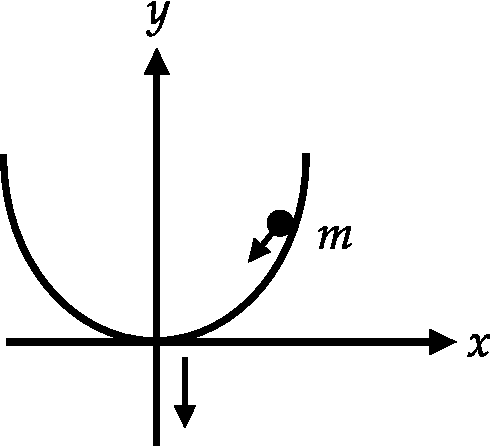
\includegraphics[height=3.5cm,width=4cm]{diagram-20210915(2)-crop}
	\end{figure}
	The Lagrangian for this particle is given by
	{	\exyear{GATE 2012}}
	\begin{tasks}(2)
		\task[\textbf{A.}] $L=\frac{1}{2} m \dot{x}^{2}-m g a x^{2}$
		\task[\textbf{B.}] $L=\frac{1}{2} m\left(1+4 a^{2} x^{2}\right) \dot{x}^{2}-m g a x^{2}$
		\task[\textbf{C.}] $L=\frac{1}{2} m \dot{x}^{2}+m g a x^{2}$
		\task[\textbf{D.}] $L=\frac{1}{2} m\left(1+4 a^{2} x^{2}\right) \dot{x}^{2}+m g a x^{2}$
	\end{tasks}
\begin{answer}
	\begin{align*}
	\text{	Equation of constrain is given by }y&=a x^{2}, K.E., T=\frac{1}{2}m\left(\dot{x}^{2}+\dot{y}^{2}\right)\\
	\dot{y}&=2 a x \dot{x} \Rightarrow T=\frac{1}{2} m\left(\dot{x}^{2}+4 a^{2} x^{2} \dot{x}^{2}\right)\\&=\frac{1}{2} m \dot{x}^{2}\left(1+4 a x^{2}\right) \\
	V&=m g y=m g a x^{2}\\
	\because L&=T-V \Rightarrow L\\&=\frac{1}{2} m\left(1+4 a^{2} x^{2}\right) \dot{x}^{2}-m g a x^{2}
	\end{align*}
	So the correct answer is \textbf{Option (B)}
\end{answer}
	\item  The Lagrange's equation of motion of the particle for above question is given by
	{\exyear{GATE 2012}}
	\begin{tasks}(1)
		\task[\textbf{A.}] $\ddot{x}=2 g a x$
		\task[\textbf{B.}] $m\left(1+4 a^{2} x^{2}\right) \ddot{x}=-2 m g a x-4 m a^{2} x \dot{x}^{2}$
		\task[\textbf{C.}] $m\left(1+4 a^{2} x^{2}\right) \ddot{x}=2 m g a x+4 m a^{2} x \dot{x}^{2}$
		\task[\textbf{D.}] $\ddot{x}=-2 g a x$
	\end{tasks}
\begin{answer}
	\begin{align*}
	\frac{d}{d t}\left(\frac{d L}{d \dot{x}}\right)&=\frac{d L}{d x} \Rightarrow m \ddot{x}\left(1+4 a^{2} x^{2}\right)\\&=-4 m a^{2} x \dot{x}^{2}-2 m g a x
	\end{align*}
	So the correct answer is \textbf{Option (B)}
\end{answer}
	\item The Lagrangian of a system with one degree of freedom $q$ is given by $L=\alpha \dot{q}^{2}+\beta q^{2}$, where $\alpha$ and $\beta$ are non-zero constants. If $p_{q}$ denotes the canonical momentum conjugate to $q$ then which one of the following statements is CORRECT?
	{\exyear{GATE 2013}}
	\begin{tasks}(1)
		\task[\textbf{A.}] $p_{q}=2 \beta q$ and it is a conserved quantity.
		\task[\textbf{B.}]  $p_{q}=2 \beta q$ and it is not a conserved quantity.
		\task[\textbf{C.}] $p_{q}=2 \alpha \dot{q}$ and it is a conserved quantity.
		\task[\textbf{D.}]  $p_{q}=2 \alpha \dot{q}$ and it is not a conserved quantity.
	\end{tasks}
\begin{answer}
	\begin{align*}
	\text{	As, }\frac{\partial L}{\partial \dot{q}}=p_{q}\text{ but }\quad \frac{\partial L}{\partial q} \neq 0.\text{ Thus, it is not a conserved quantity.}
	\end{align*}
	So the correct answer is \textbf{Option (D)}
\end{answer}
	\item A bead of mass $m$ can slide without friction along a massless rod kept at $45^{\circ}$ with the vertical as shown in the figure. The rod is rotating about the vertical axis with a constant angular speed $\omega$. At any instant $r$ is the distance of the bead from the origin. The momentum conjugate to $r$ is
	{\exyear{GATE 2014}}
	\begin{figure}[H]
		\centering
		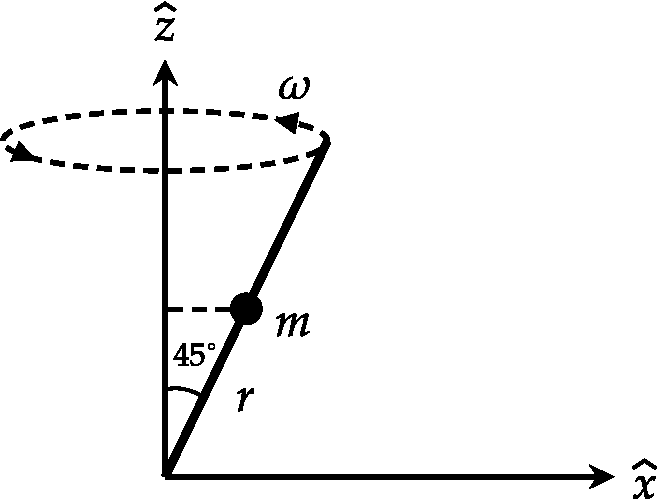
\includegraphics[height=3.5cm,width=5cm]{diagram-20210915(4)-crop}
	\end{figure}
	\begin{tasks}(4)
		\task[\textbf{A.}] $m \dot{r}$
		\task[\textbf{B.}] $\frac{1}{\sqrt{2}} m \dot{r}$
		\task[\textbf{C.}] $\frac{1}{2} m \dot{r}$
		\task[\textbf{D.}] $\sqrt{2} m \dot{r}$
	\end{tasks}
\begin{answer}
	\begin{align*}
	L&=\frac{1}{2} m\left(\dot{r}^{2}+r^{2} \dot{\theta}^{2}+r^{2} \sin ^{2} \theta \dot{\phi}^{2}\right)-m g r \cos \theta\\
	\text{Equation of constrain is }\theta&=\frac{\pi}{4}\text{ and it is given } \dot{\phi}=\omega\\
	L&=\frac{1}{2} m\left(\dot{r}^{2}+\frac{1}{2} r^{2} \omega^{2}\right)-\frac{1}{\sqrt{2}} m g r\\
	\text{	Thus the momentum conjugate to $r$ is }p_{r}&=\frac{\partial L}{\partial \dot{r}} \Rightarrow p_{r}=m \dot{r}
	\end{align*}
	So the correct answer is \textbf{Option (A)}
\end{answer}
	\item The Lagrangian of a system is given by
	$L=\frac{1}{2} m l^{2}\left[\dot{\theta}^{2}+\sin ^{2} \theta \dot{\varphi}^{2}\right]-m g l \cos \theta$, where $m, l$ and $g$ are constants.
	Which of the following is conserved?
	{\exyear{GATE 2016}}
	\begin{tasks}(4)
		\task[\textbf{A.}] $\dot{\varphi} \sin ^{2} \theta$
		\task[\textbf{B.}] $\dot{\varphi} \sin \theta$
		\task[\textbf{C.}] $\frac{\dot{\varphi}}{\sin \theta}$
		\task[\textbf{D.}] $\frac{\dot{\varphi}}{\sin ^{2} \theta}$
	\end{tasks}
\begin{answer}
	\begin{align*}
	\intertext{Solution: As $\varphi$ is cyclic coordinate, so $\frac{\partial L}{\partial \dot{\varphi}}=p_{\varphi}=m l^{2} \sin ^{2} \dot{\varphi}$, is a constant since $m, l$ and $g$ are constants. Thus $\dot{\varphi} \sin ^{2} \theta$ is conserved.}
	\end{align*}
	So the correct answer is \textbf{Option (A)}
\end{answer}
	\item If the Lagrangian $L_{0}=\frac{1}{2} m\left(\frac{d q}{d t}\right)^{2}-\frac{1}{2} m \omega^{2} q^{2}$ is modified to $L=L_{0}+\alpha q\left(\frac{d q}{d t}\right)$, which one of the following is TRUE?
	{\exyear{GATE 2017}}
	\begin{tasks}(1)
		\task[\textbf{A.}] Both the canonical momentum and equation of motion do not change
		\task[\textbf{B.}] Canonical momentum changes, equation of motion does not change
		\task[\textbf{C.}] Canonical momentum does not change, equation of motion changes
		\task[\textbf{D.}] Both the canonical momentum and equation of motion change
	\end{tasks}
\begin{answer}
	\begin{align*}
	\text{	For Lagrangian }L_{0}&=\frac{1}{2} m\left(\frac{d q}{d t}\right)^{2}-\frac{1}{2} m \omega^{2} q^{2}\\
	\text{canonical momentum is }p&=m \dot{q}
	\intertext{ and equation of motion is given by }\frac{d}{d t}\left(\frac{\partial L}{\partial \dot{q}}\right)-\left(\frac{\partial L}{\partial q}\right)&=0 \Rightarrow m \ddot{q}+m \omega^{2} q=0\\
	\text{For Lagrangian }L&=L_{0}+\alpha q\left(\frac{d q}{d t}\right) \Rightarrow L\\&=\frac{1}{2} m\left(\frac{d q}{d t}\right)^{2}-\frac{1}{2} m \omega^{2} q^{2}+\alpha q \dot{q}\\
	\text{Canonical momentum is }p&=m \dot{q}+\alpha q\\
	\text{Equation of motion is,}\\
	\frac{d}{d t}\left(\frac{\partial L}{\partial \dot{q}}\right)-\left(\frac{\partial L}{\partial q}\right)&=0 \Rightarrow m \ddot{q}+m \omega^{2} q=0
	\end{align*}
	So the correct answer is \textbf{Option (B)}
\end{answer}
	\item  A double pendulum consists of two equal masses $m$ suspended by two strings of length $l$. What is the Lagrangian of this system for oscillations in a plane? Assume the angles $\theta_{1}, \theta_{2}$ made by the two strings are small (you can use $\cos \theta=1-\theta^{2} / 2$ ).\\
	Note: $\omega_{0}=\sqrt{g / l}$.
	{\exyear{JEST 2014}}
	\begin{tasks}(1)
		\task[\textbf{A.}] $L \approx m l^{2}\left(\dot{\theta}_{1}^{2}+\frac{1}{2} \dot{\theta}_{2}^{2}-\omega_{0}^{2} \theta_{1}^{2}-\frac{1}{2} \omega_{0}^{2} \theta_{2}^{2}\right)$
		\task[\textbf{B.}]  $L \approx m l^{2}\left(\dot{\theta}_{1}^{2}+\frac{1}{2} \dot{\theta}_{2}^{2}+\dot{\theta}_{1} \dot{\theta}_{2}-\omega_{0}^{2} \theta_{1}^{2}-\frac{1}{2} \omega_{0}^{2} \theta_{2}^{2}\right)$
		\task[\textbf{C.}] $L \approx m l^{2}\left(\dot{\theta}_{1}^{2}+\frac{1}{2} \dot{\theta}_{2}^{2}-\dot{\theta}_{1} \dot{\theta}_{2}-\omega_{0}^{2} \theta_{1}^{2}-\frac{1}{2} \omega_{0}^{2} \theta_{2}^{2}\right)$
		\task[\textbf{D.}]  $L \approx m l^{2}\left(\frac{1}{2} \dot{\theta}_{1}^{2}+\frac{1}{2} \dot{\theta}_{2}^{2}+\dot{\theta}_{1} \dot{\theta}_{2}-\omega_{0}^{2} \theta_{1}^{2}-\omega_{0}^{2} \theta_{2}^{2}\right)$
	\end{tasks}
\begin{answer}$\left. \right. $\\
	\begin{minipage}{0.45\textwidth}
		\begin{align*}
		x_{1}&=l \sin \theta_{1},\\ y_{1}&=l \cos \theta_{1}\\
		x_{2}&=x_{1}+l \sin \theta_{2}\\y_{2}&=y_{1}+l \cos \theta_{2}\\
		\dot{x}_{2}&=l \cos \theta_{1} \dot{\theta}_{1}+l \cos \theta_{2} \dot{\theta}_{2},\\ \dot{y}_{2}&=-l \sin \theta_{1} \dot{\theta}_{1}-l \sin \theta_{2} \dot{\theta}_{2}\\
		\dot{x}_{2}^{2}+\dot{y}_{2}^{2}&=l^{2} \cos ^{2} \theta_{1} \dot{\theta}_{1}^{2}+l^{2} \cos ^{2} \theta_{2} \dot{\theta}_{2}^{2}\\&+2 l^{2} \cos \theta_{1} \dot{\theta}_{1} \cos \theta_{2} \dot{\theta}_{2}+l^{2} \sin \theta_{1}^{2} \dot{\theta}_{1}^{2}
		\\&+l^{2} \sin \theta_{2}^{2} \dot{\theta}_{2}^{2}+2 l^{2} \sin \theta_{1} \sin \theta_{2} \dot{\theta}_{1} \dot{\theta}_{2}\\
		\Rightarrow \dot{x}_{2}^{2}+\dot{y}_{2}^{2}&=l^{2} \dot{\theta}_{1}^{2}+l^{2} \dot{\theta}_{2}^{2}+2 l^{2} \cos \left(\theta_{1}-\theta_{2}\right) \dot{\theta}_{1} \dot{\theta}_{2}\\\text{ also }\dot{x}_{1}^{2}+\dot{y}_{1}^{2}&=l^{2} \dot{\theta}_{1}^{2}\\
		\end{align*}
	\end{minipage}
	\begin{minipage}{0.35\textwidth}
		\begin{figure}[H]
			\centering
			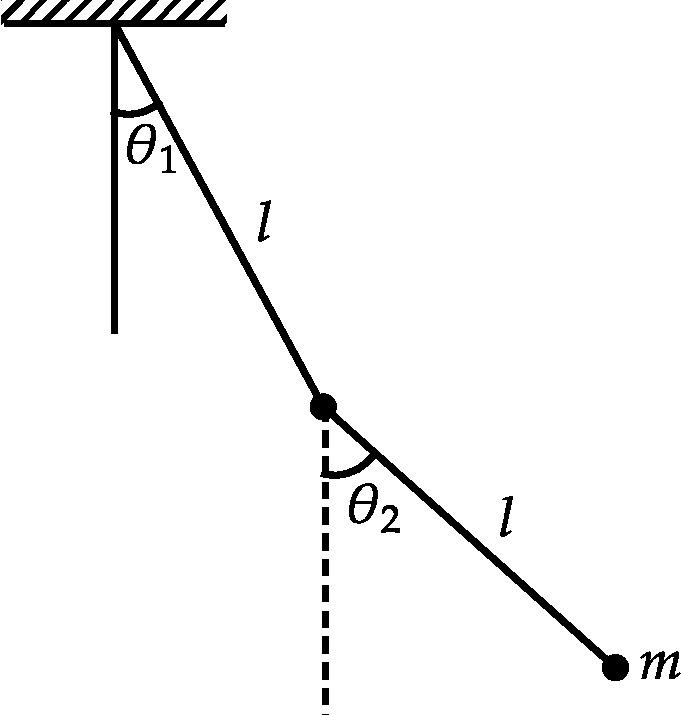
\includegraphics[height=4cm,width=4cm]{diagram-20210807(4)-crop}
		\end{figure}
	\end{minipage}
	\begin{align*}
	L=T-V&=\frac{1}{2} m\left(\dot{x}_{1}^{2}+\dot{y}_{1}^{2}+\dot{x}_{2}^{2}+\dot{y}_{2}^{2}\right)-m g y_{1}-m g y_{2}\\
	\Rightarrow L&=\frac{1}{2} m\left(l^{2} \dot{\theta}_{1}^{2}+l^{2} \dot{\theta}_{1}^{2}+l^{2} \dot{\theta}_{2}^{2}+2 l^{2} \cos \left(\theta_{1}-\theta_{2}\right) \dot{\theta}_{1} \dot{\theta}_{2}\right)\\&+2 m g l \cos \theta_{1}+m g l \cos \theta_{2}\\
	\Rightarrow L&=m l^{2}\left[\dot{\theta}_{1}^{2}+\frac{1}{2} \dot{\theta}_{2}^{2}+\dot{\theta}_{1} \dot{\theta}_{2}+\frac{2 g}{2 l}\left(1-\frac{\theta_{1}^{2}}{2}\right)+\frac{1}{2} \frac{g}{l}\left(1-\frac{\theta_{2}^{2}}{2}\right)\right]\\&\left[\because \cos \left(\theta_{1}-\theta_{2}\right) \approx 1\right]\\
	\Rightarrow L&=m l^{2}\left[\dot{\theta}_{1}^{2}+\frac{1}{2} \dot{\theta}_{2}^{2}+\dot{\theta}_{1} \dot{\theta}_{2}+\frac{g}{l}-\frac{g}{l} \frac{\theta_{1}^{2}}{2}+\frac{g}{2 l}-\frac{g}{2 l} \frac{\theta_{2}^{2}}{2}\right]
	\intertext{comparing given options, option (B) is correct i.e.}
	L&=m l^{2}\left(\dot{\theta}_{1}^{2}+\frac{1}{2} \dot{\theta}_{2}^{2}+\dot{\theta}_{1} \dot{\theta}_{2}-\frac{\omega_{0}^{2} \dot{\theta}_{1}^{2}}{2}-\frac{1}{4} \omega_{0} \dot{\theta}_{2}^{2}\right)
	\end{align*}
	So the correct answer is \textbf{Option (B)}
\end{answer}
	\item A bike stuntman rides inside a well of frictionless surface given by $z=a\left(x^{2}+y^{2}\right)$, under the action of gravity acting in the negative $z$ direction. $\vec{g}=-g \hat{z} .$ What speed should be maintain to be able to ride at a constant height $z_{0}$ without falling down?
	{\exyear{JEST 2015}}
	\begin{tasks}(1)
		\task[\textbf{A.}] $\sqrt{g z_{0}}$
		\task[\textbf{B.}] $\sqrt{3 g z_{0}}$
		\task[\textbf{C.}] $\sqrt{2 g z_{0}}$
		\task[\textbf{D.}] The biker will not be able to maintain a constant height, irrespective of speed.
	\end{tasks}
\begin{answer}
	\begin{align*}
	z&=a\left(x^{2}+y^{2}\right)
	\intertext{Using equation of constrain, we must solve the given system in cylindrical co-ordinate.}
	z&=a r^{2}, \dot{z}=2 a r \dot{r} \Rightarrow L\\&=\frac{1}{2} m\left(\dot{r}^{2}+r^{2} \dot{\theta}+\dot{z}^{2}\right)-m g z\\
	\Rightarrow L&=\frac{1}{2} m\left(\dot{r}^{2}+r^{2} \dot{\theta}+4 a^{2} r^{2} \dot{r}^{2}\right)-m g a r^{2}\\&=\frac{1}{2} m\left[\dot{r}^{2}\left(1+4 a^{2} r^{2}\right)+r^{2} \dot{\theta}^{2}\right]-m g a r^{2}\\
	\text{	Equation of motion}\\
	\frac{d}{d t}\left(\frac{\partial L}{\partial \dot{r}}\right)-\frac{\partial L}{\partial r}&=0\\
	\Rightarrow m \ddot{r}\left(1+4 a^{2} r^{2}\right)+m \dot{r}^{2} 4 a^{2} r-m r \dot{\theta}^{2}+2 m g a r&=0\\
	\text{At }z=z_{0}, \dot{r}=0, \quad r=r_{0},\text{ so,} m r_{0} \dot{\theta}^{2}&=2 m g a r_{0}\\
	\dot{\theta}^{2}&=2 g a \Rightarrow \dot{\theta}=\sqrt{2 g a}, \frac{v}{r_{0}}\\&=\sqrt{2 g a}, v=\sqrt{2 g a} \cdot r_{0}\\
	v&=\sqrt{2 g a} \cdot\left(\frac{z_{0}}{a}\right)^{1 / 2}\\&=\sqrt{2 g z_{0}}\\
	\left(\because z_{0}=a r_{0}^{2}\right)
	\end{align*}
	\begin{figure}[H]
		\centering
		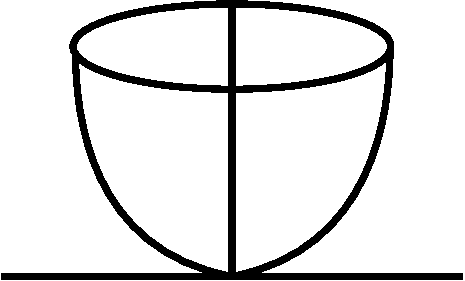
\includegraphics[height=2.5cm,width=4cm]{diagram-20210809(8)-crop}
	\end{figure}
	So the correct answer is \textbf{Option (C)}
\end{answer}
	\item The Lagrangian of a particle is given by $L=\dot{q}^{2}-q \dot{q}$. Which of the following statements is true?
	{\exyear{JEST 2015}}
	\begin{tasks}(1)
		\task[\textbf{A.}]  This is a free particle
		\task[\textbf{B.}] The particle is experiencing velocity dependent damping
		\task[\textbf{C.}] The particle is executing simple harmonic motion
		\task[\textbf{D.}] The particle is under constant acceleration.
	\end{tasks}
\begin{answer}
	\begin{align*}
	\because L&=\dot{q}^{2}-q \dot{q} \Rightarrow \frac{\partial L}{\partial \dot{q}}\\&=2 \dot{q}-q \Rightarrow \frac{d}{d t}\left(\frac{\partial L}{\partial \dot{q}}\right)\\&=2 \ddot{q}-\dot{q}\\
	\because \frac{d}{d t}\left(\frac{\partial L}{\partial \dot{q}}\right)-\frac{\partial L}{\partial q}&=0
	\Rightarrow 2 \ddot{q}-\dot{q}+\dot{q}\\&=0 \Rightarrow 2 \ddot{q}=0 \Rightarrow \frac{d^{2} q}{d t^{2}}\\&=0 \Rightarrow \frac{d q}{d t}=C \Rightarrow q=C t+\alpha
	\end{align*}
	So the correct answer is \textbf{Option (A)}
\end{answer}
	\item A hoop of radius a rotates with constant angular velocity $\omega$ about the
	vertical axis as shown in the figure. A bead of mass $m$ can slide on the
	hoop without friction. If $g<\omega^{2} a$ at what angle $\theta$ apart from 0 and $\pi$ is the bead stationary (i.e., $\frac{d \theta}{d t}=\frac{d^{2} \theta}{d t^{2}}=0$ )?
	{\exyear{JEST 2016}}
	\begin{figure}[H]
		\centering
		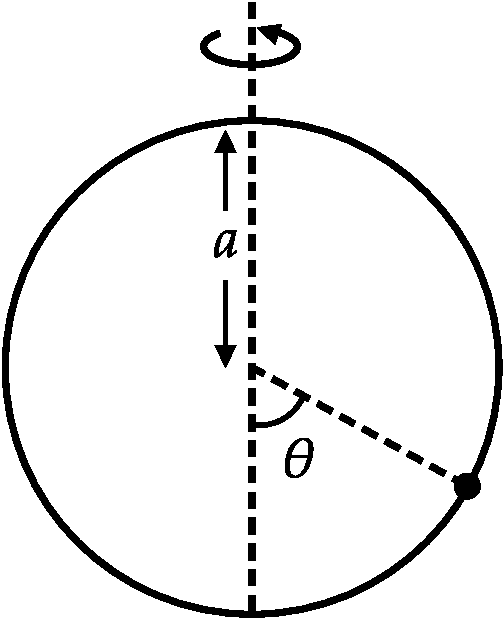
\includegraphics[height=4.2cm,width=3.5cm]{diagram-20210809(11)-crop}
	\end{figure}
	\begin{tasks}(4)
		\task[\textbf{A.}] $\tan \theta=\frac{\pi g}{\omega^{2} a}$
		\task[\textbf{B.}] $\sin \theta=\frac{g}{\omega^{2} a}$
		\task[\textbf{C.}] $\cos \theta=\frac{g}{\omega^{2} a}$
		\task[\textbf{D.}] $\tan \theta=\frac{g}{\pi \omega^{2} a}$
	\end{tasks}
\begin{answer}
	\begin{align*}
	\text{The Lagrangian of the system is}\\
	L&=\frac{1}{2} m a^{2}\left(\dot{\theta}^{2}+\sin ^{2} \theta \dot{\phi}^{2}\right)+m g a \cos \theta\\
	\text{The equation of motion is,}\\
	&\frac{d}{d t}\left(\frac{\partial L}{\partial \dot{\theta}}\right)-\left(\frac{\partial L}{\partial \theta}\right)\\&=0 \Rightarrow m a^{2} \ddot{\theta}-m a^{2}\left(\sin \theta \cos \theta \dot{\phi}^{2}\right)+m g a \sin \theta=0\\
	\text{When bead is stationary, then}\\
	\frac{d \theta}{d t}&=\frac{d^{2} \theta}{d t^{2}}\\&=0 \Rightarrow-m a^{2}\left(\sin \theta \cos \theta \dot{\phi}^{2}\right)+m g a \sin \theta=0\\
	\Rightarrow \dot{\phi}&=\omega\text{ and }g<\omega^{2} a,\text{ then }\cos \theta=\frac{g}{\omega^{2} a}
	\end{align*}
	So the correct answer is \textbf{Option (C)}
\end{answer}
	\item A bead of mass $M$ slides along a parabolic wire described by $z=2\left(x^{2}+y^{2}\right)$. The wire rotates with angular velocity $\Omega$ about the $z$ - axis. At what value of $\Omega$ does the bead maintain a constant nonzero height under the action of gravity along $-\hat{z}$ ?
	{\exyear{JEST 2017}}
	\begin{tasks}(4)
		\task[\textbf{A.}] $\sqrt{3 g}$
		\task[\textbf{B.}] $\sqrt{g}$
		\task[\textbf{C.}] $\sqrt{2 g}$
		\task[\textbf{D.}] $\sqrt{4 g}$
	\end{tasks}
\begin{answer}
	\begin{align*}
	L&=\frac{1}{2} m\left(\dot{r}^{2}+r^{2} \dot{\theta}^{2}+16 r^{2} \dot{r}^{2}\right)-2 m g r^{2} \Rightarrow L\\&=\frac{1}{2} m\left(\dot{r}^{2}\left(1+16 r^{2}\right)+r^{2} \dot{\theta}^{2}\right)-2 m g r^{2}
	\intertext{The equation of motion is given by}
	&\frac{d}{d t}\left(\frac{\partial L}{\partial \dot{r}}\right)-\frac{\partial L}{\partial r}\\&=0 \Rightarrow m \ddot{r}\left(1+16 r^{2}\right)+16 m \dot{r}^{2} r-m r \dot{\theta}^{2}+4 m g r=0\\
	\text{	At equilibrium, }r&=r_{0}, \dot{r}=0, \ddot{r}=0\\
	\text{So, }-m r_{0} \dot{\theta}^{2}+4 m g r_{0}&=0 \Rightarrow \dot{\theta}=\Omega=\sqrt{4 g}
	\end{align*}
	So the correct answer is \textbf{Option (D)}
\end{answer}
	\item A possible Lagrangian for a free particle is
	{\exyear{JEST 2017}}
	\begin{tasks}(4)
		\task[\textbf{A.}] $L=\dot{q}^{2}-q^{2}$
		\task[\textbf{B.}] $L=\dot{q}^{2}-q \dot{q}$
		\task[\textbf{C.}] $L=\dot{q}^{2}-q$
		\task[\textbf{D.}] $L=\dot{q}^{2}-\frac{1}{q}$
	\end{tasks}
\begin{answer}
	\begin{align*}
	\frac{d}{d t}\left(\frac{\partial L}{\partial \dot{q}}\right)-\left(\frac{\partial L}{\partial q}\right)&=0 \Rightarrow 2 \ddot{q}-\dot{q}+\dot{q}\\&=0 \Rightarrow \ddot{q}=0
	\end{align*}
	So the correct answer is \textbf{Option (B)}
\end{answer}
	\item  A rod of mass $m$ and length $l$ is suspended from two massless vertical springs with a spring constants $k_{1}$ and $k_{2} .$ What is the Lagrangian for the system, if $x_{1}$ and $x_{2}$ be the displacements from equilibrium position of the two ends of the rod?
	{\exyear{JEST 2017}}
	\begin{tasks}(1)
		\task[\textbf{A.}] $\frac{m}{8}\left(\dot{x}_{1}^{2}+2 \dot{x}_{1} \dot{x}_{2}+\dot{x}_{2}^{2}\right)-\frac{1}{2} k_{1} x_{1}^{2}-\frac{1}{2} k_{2} x_{2}^{2}$
		\task[\textbf{B.}] $\frac{m}{2}\left(\dot{x}_{1}^{2}+\dot{x}_{1} \dot{x}_{2}+\dot{x}_{2}^{2}\right)-\frac{1}{4}\left(k_{1}+k_{2}\right)\left(x_{1}^{2}+x_{2}^{2}\right)$
		\task[\textbf{C.}] $\frac{m}{6}\left(\dot{x}_{1}^{2}+x_{1} \dot{x}_{2}+\dot{x}_{2}^{2}\right)-\frac{1}{2} k_{1} x_{1}^{2}-\frac{1}{2} k_{2} x_{2}^{2}$
		\task[\textbf{D.}] $\frac{m}{2}\left(\dot{x}_{1}^{2}-2 \dot{x}_{1} \dot{x}_{2}+\dot{x}_{2}^{2}\right)-\frac{1}{4}\left(k_{1}-k_{2}\right)\left(x_{1}^{2}+x_{2}^{2}\right)$
	\end{tasks}
\begin{answer}
	\begin{align*}
	T&=\frac{1}{2} M V_{c, m}^{2}+\frac{1}{2} I_{c . m} \omega^{2}\\&=\frac{1}{2} m\left(\frac{\dot{x}_{1}+\dot{x}_{2}}{2}\right)^{2}+\frac{1}{2} \frac{m l^{2}}{12} \dot{\theta}^{2}\\
	\text{	Potential energy is, }V&=\frac{1}{2} k x_{1}^{2}+\frac{1}{2} k x_{2}^{2}\\
	\sin \theta&=\frac{x_{2}-x_{1}}{l}\text{ for small oscillation} \theta\\&=\frac{x_{2}-x_{1}}{l}=\dot{\theta}\\&=\frac{\dot{x}_{2}-\dot{x}_{1}}{l}\\
	L&=\frac{1}{2} m\left(\frac{\dot{x}_{1}+\dot{x}_{2}}{2}\right)^{2}+\frac{1}{2} \frac{m l^{2}}{12}\left(\frac{\dot{x}_{1}-\dot{x}_{2}}{l}\right)^{2}-\frac{1}{2} k x_{1}^{2}-\frac{1}{2} k x_{2}^{2}\\
	&=\frac{m}{6}\left(\dot{x}_{1}^{2}+x_{1} \dot{x}_{2}+\dot{x}_{2}^{2}\right)-\frac{1}{2} k_{1} x_{1}^{2}-\frac{1}{2} k_{2} x_{2}^{2}
	\end{align*}
	So the correct answer is \textbf{Option (C)}
\end{answer}
	\item Consider the Lagrangian
	$$L=1-\sqrt{1-\dot{q}^{2}}-\frac{q^{2}}{2}$$
	of a particle executing oscillations whose amplitude is $A$. If $p$ denotes the momentum of the particle, then $4 p^{2}$ is
	{\exyear{JEST 2015}}
	\begin{tasks}(2)
		\task[\textbf{A.}] (a) $\left(A^{2}-q^{2}\right)\left(4+A^{2}-q^{2}\right)$
		\task[\textbf{B.}] $\left(A^{2}+q^{2}\right)\left(4+A^{2}-q^{2}\right)$
		\task[\textbf{C.}] $\left(A^{2}-q^{2}\right)\left(4+A^{2}+q^{2}\right)$
		\task[\textbf{D.}] $\left(A^{2}+q^{2}\right)\left(4+A^{2}+q^{2}\right)$
	\end{tasks}	
\begin{answer}
	So the correct answer is \textbf{Option (A)}
\end{answer}
	\item Consider the motion of a particle in two dimensions given by the Lagrangian $$L=\frac{m}{2}\left(\dot{x}^{2}+\dot{y}^{2}\right)-\frac{\lambda}{4}(x+y)^{2}$$
	where $\lambda>0$. The initial conditions are given as $y(0)=0, x(0)=42$ meters, $\dot{x}(0)=\dot{y}(0)=0$. What is the value of $x(t)-y(t)$ at $t=25$ seconds in meters?
	{\exyear{JEST 2019}}
	\begin{answer}
		\begin{align}
		L&=\frac{m}{2}\left(\dot{x}^{2}+\dot{y}^{2}\right)-\frac{\lambda}{4}(x+y)^{2}\notag
		\intertext{The equation of motion is}
		\frac{d}{d t}\left(\frac{\partial L}{\partial \dot{x}}\right)-\left(\frac{\partial L}{\partial x}\right)&=0 \Rightarrow m \ddot{x}+\frac{\lambda}{2} x+\frac{\lambda}{2} y=0\label{72-1}\\
		\frac{d}{d t}\left(\frac{\partial L}{\partial \dot{y}}\right)-\left(\frac{\partial L}{\partial y}\right)&=0 \Rightarrow m \ddot{y}+\frac{\lambda}{2} y+\frac{\lambda}{2} x=0\label{72-2}
		\intertext{Subtracting equation (\ref{72-1}) from (\ref{72-2}) gives $m(\ddot{x}-\ddot{y})=0 \Rightarrow \ddot{x}-\ddot{y}=0$}\notag
		\intertext{Integrating both sides with $t$ gives}\notag
		\dot{x}-\dot{y}&=c_{1}\notag\\
		\text{	From the equation }\dot{x}(0)&=\dot{y}(0)=0,\text{ there }c_{1}=0\notag\\
		\text{Hence, }\dot{x}-\dot{y}&=0\label{jest10}\\
		\intertext{Integrating both sides of this equation with $t$ gives}
		x-y&=c_{2}\notag\\
		\text{Putting }x(0)&=42, y(0)=0\text{ gives}\notag\\
		42-0&=c_{2} \Rightarrow 42\notag\\
		\text{Therefore, }x-y=42\notag\\
		\intertext{The value of $x-y$ is independent of $t$.}\notag
		\text{Therefore, at }t&=25 s\notag\\
		x(t)-y(t)&=42\notag
		\end{align}
	\end{answer}
\end{enumerate}
\colorlet{ocre1}{ocre!70!}
\colorlet{ocrel}{ocre!30!}
\setlength\arrayrulewidth{1pt}
\begin{table}[H]
	\centering
	\arrayrulecolor{ocre}
	\begin{tabular}{|p{1.5cm}|p{1.5cm}||p{1.5cm}|p{1.5cm}|}
		\hline
		\multicolumn{4}{|c|}{\textbf{Answer key}}\\\hline\hline
		\rowcolor{ocrel}Q.No.&Answer&Q.No.&Answer\\\hline
		1&\textbf{B} &2&\textbf{B}\\\hline 
		3&\textbf{D} &4&\textbf{A} \\\hline
		5&\textbf{A} &6&\textbf{B} \\\hline
		7&\textbf{B}&8&\textbf{C}\\\hline
		9&\textbf{A}&10&\textbf{C}\\\hline
		11&\textbf{D} &12&\textbf{B}\\\hline
		13&\textbf{C}&14&\textbf{A}\\\hline
		15&\textbf{42}& &\\\hline
		
	\end{tabular}
\end{table}